\chapter{Opdracht week 4}

\section{Toepassing 1}

Als eerste werd er natuurlijk gedacht aan het originele idee,
een website waarop services gedeeld en ingehuurd worden.

\subsection{Relatie SWOT}
{\bf Hoe zijn we op dit idee gekomen, hoe is dit gerelateerd}

\subsection{Uitbreidingsplan}

\subsubsection{Doel}
{\bf Bedoeling met het systeem, welke partijen hebben er mee te maken}

\subsubsection{Impact}
{\bf Wat is er nodig, wat gebeurt er met het bedrijf}

Hieronder is een simpel voorbeeld van de onderliggende architectuur.

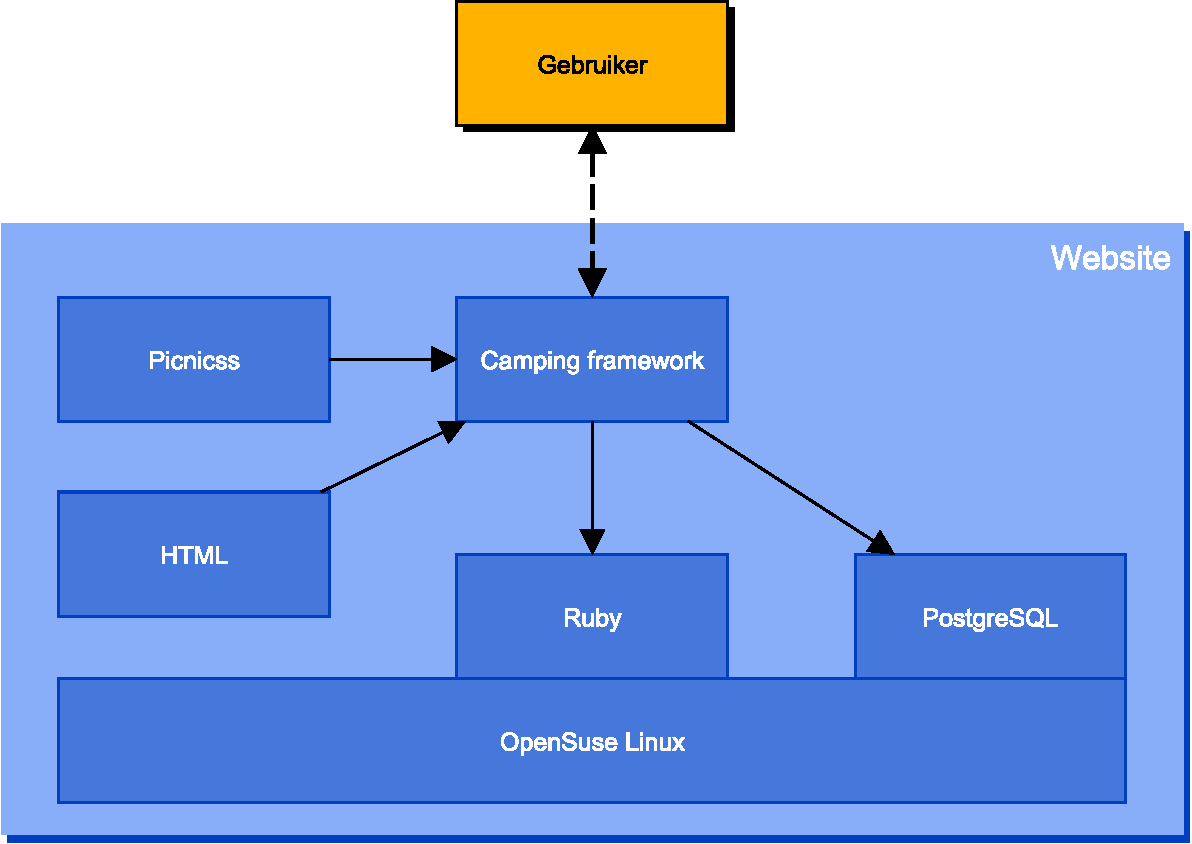
\includegraphics[width=\textwidth]{img/websiteArchitecture}

\subsubsection{Omschrijving}
{\bf Systeemontwerpen, wireframes, designs}

\section{Toepassing 2}

Een app zou eenzelfde soort functie kunnen leveren,
maar zal andere mensen aantrekken.
Een hypothese zou kunnen zijn dat een app het gemak verhoogd
en dus de markt groter maakt,
met een breder scala aan mensen.

\subsection{Relatie SWOT}
{\bf Hoe zijn we op dit idee gekomen, hoe is dit gerelateerd}

\subsection{Uitbreidingsplan}

\subsubsection{Doel}
{\bf Bedoeling met het systeem, welke partijen hebben er mee te maken}

\subsubsection{Impact}
{\bf Wat is er nodig, wat gebeurt er met het bedrijf}

\subsubsection{Omschrijving}
{\bf Systeemontwerpen, wireframes, designs}

\section{Toepassing 3}

Gezien we een handjevol competente ICT Beheerders in de groep hebben,
is het normaal om de benodigde ICT-gerelateerde services zelf te beheren.
Omdat er een grote kans is dat er meerdere servers benodigd zullen zijn,
is het belangrijk om een goede basis te hebben.

\subsection{Relatie SWOT}
{\bf Hoe zijn we op dit idee gekomen, hoe is dit gerelateerd}

Het bedrijf is gefocused op snelle communicatie,
hiervoor is een stabiel platform erg belangrijk.
Dit systeem zorgt er ook voor dat systeembeheerders meer 'agile' kunnen werken.
Dit zorgt ervoor dat we als klein bedrijf wendbaar blijven.

\subsection{Uitbreidingsplan}

\subsubsection{Doel}
{\bf Bedoeling met het systeem, welke partijen hebben er mee te maken}

Dit systeem moet er voor zorgen dat het beheren van alle servers in het bedrijf
makkelijker en beter schaalbaar wordt door een deel ervan te automatiseren.
Daarom is dit systeem een groot voordeel voor systeembeheerders binnen het bedrijf.

Gezien de website van het bedrijf op Linux zal worden gedraaid,
zal dit systeem ook op Linux draaien.
Om ervoor te zorgen dat er snel nieuwe servers op kunnen worden gezet,
word er een hypervisor ingezet samen met een configuration management server.

\subsubsection{Impact}
{\bf Wat is er nodig, wat gebeurt er met het bedrijf}

Voor het implementeren van dit systeem zal er minimaal 1 systeembeheerder nodig zijn.
Voor een enkele systeembeheerder met kennis van zoiets dergelijks
zal het implementeren hiervan ongeveer 2-3 weken kosten, sprekende uit ervaring
van 1 van systeembeheerders.

\subsubsection{Omschrijving}
{\bf Systeemontwerpen, wireframes, designs}
